
\section{The Canonical Decomposition-Recombination Plan}

\subsection{Theory}

% \begin{figure*}\centering
% \begin{tikzpicture}
%     \tikzstyle{v}=[draw, circle, minimum size=0.75cm]
%     \tikzstyle{e}=[]

%     \node[v] (v1) at (1,1) {$R_j$};
%     \node[v] (v2) at (3,1) {$R_k$};
%     \node[v] (v3) at (2,2) {$D$};
%     \node[v] (v4) at (2,3.3) {$R_i$};

%     \tedge{v1}{v3}{solid}{}{above};
%     \tedge{v2}{v3}{solid}{}{above};
%     \tedge{v3}{v4}{solid}{}{right};
% \end{tikzpicture}
% \ldots with weights \ldots
% \begin{tikzpicture}
%     \tikzstyle{v}=[draw, circle, minimum size=0.75cm]
%     \tikzstyle{e}=[]

%     \node[v] (v1) at (1,1) {y};
%     \node[v] (v2) at (3,1) {z};
%     \node[v] (v3) at (2,2) {k};
%     \node[v] (v4) at (2,3.3) {x};

%     \tedge{v1}{v3}{solid}{y}{above};
%     \tedge{v2}{v3}{solid}{z}{above};
%     \tedge{v3}{v4}{solid}{x}{right};

%     % \draw (3.3,2.5) circle (1.9cm);
%     % \draw (.7,2.5) circle (1.9cm);
%     % \draw (2,.5) circle (1.9cm);
% \end{tikzpicture}
% \\
% \begin{tikzpicture}
%     \tikzstyle{v}=[draw, circle, minimum size=0.75cm]
%     \tikzstyle{e}=[]

%     \node[v] (v1) at (0,  0) {kxyz};
%     \node[v] (v2) at (-1,-1) {kxy};
%     \node[v] (v3) at ( 1,-1) {kyz};
%     \node[v] (v4) at (-2,-2) {kx};
%     \node[v] (v5) at ( 0,-2) {ky};
%     \node[v] (v6) at ( 2,-2) {kz};

%     \tedge{v1}{v2}{solid}{}{};
%     \tedge{v1}{v3}{solid}{}{};
%     \tedge{v2}{v4}{solid}{}{};
%     \tedge{v2}{v5}{solid}{}{};
%     \tedge{v3}{v5}{solid}{}{};
%     \tedge{v3}{v6}{solid}{}{};
% \end{tikzpicture}
% \begin{tikzpicture}
%     \tikzstyle{v}=[draw, circle, minimum size=0.75cm]
%     \tikzstyle{e}=[]

%     \node[v] (v1) at (0,  0) {kxyz};
%     \node[v] (v2) at (-1,-1) {kxy};
%     \node[v] (v3) at ( 1,-1) {kxz};
%     \node[v] (v4) at (-2,-2) {kx};
%     \node[v] (v5) at ( 0,-2) {ky};
%     \node[v] (v6) at ( 2,-2) {kz};

%     \tedge{v1}{v2}{solid}{}{};
%     \tedge{v1}{v3}{solid}{}{};
%     \tedge{v2}{v4}{solid}{}{};
%     \tedge{v2}{v5}{solid}{}{};
%     \tedge{v3}{v4}{solid}{}{};
%     \tedge{v3}{v6}{solid}{}{};
% \end{tikzpicture}
% \begin{tikzpicture}
%     \tikzstyle{v}=[draw, circle, minimum size=0.75cm]
%     \tikzstyle{e}=[]

%     \node[v] (v1) at (0,  0) {kxyz};
%     \node[v] (v2) at (-1,-1) {kxz};
%     \node[v] (v3) at ( 1,-1) {kyz};
%     \node[v] (v4) at (-2,-2) {kx};
%     \node[v] (v5) at ( 0,-2) {ky};
%     \node[v] (v6) at ( 2,-2) {kz};

%     \tedge{v1}{v2}{solid}{}{};
%     \tedge{v1}{v3}{solid}{}{};
%     \tedge{v2}{v4}{solid}{}{};
%     \tedge{v2}{v6}{solid}{}{};
%     \tedge{v3}{v5}{solid}{}{};
%     \tedge{v3}{v6}{solid}{}{};
% \end{tikzpicture}
% % \\
% % \begin{tikzpicture}
% %     \tikzstyle{v}=[draw, circle, minimum size=0.75cm]
% %     \tikzstyle{e}=[]

% %     \node[v] (v1) at ( 0, 0) {kxyz};
% %     \node[v] (v2) at (-1,-1) {kxy};
% %     \node[v] (v3) at (-2,-2) {kx};
% %     \node[v] (v4) at (-3,-3) {k};
% %     \node[v] (v5) at ( 1,-1) {z plan};
% %     \node[v] (v6) at ( 0,-2) {y plan};
% %     \node[v] (v7) at (-1,-3) {x plan};
% %     \node[v] (v8) at (-2,-4) {k plan};

% %     \tedge{v1}{v2}{solid}{}{};
% %     \tedge{v1}{v5}{solid}{}{};
% %     \tedge{v2}{v3}{solid}{}{};
% %     \tedge{v2}{v6}{solid}{}{};
% %     \tedge{v3}{v4}{solid}{}{};
% %     \tedge{v3}{v7}{solid}{}{};
% %     \tedge{v4}{v8}{solid}{}{};
% % \end{tikzpicture}

% \caption{A well-constrained graph whose nodes are subgraphs labeled with their density. Below are its 3 optimal DR-Plans (partially complete). The center vertex has weight $k$ and is well-constrained itself. The radial nodes have weights $x,y,z \neq k$ with equivalent edge weights, making any union between $k$ and the others well-constrained. \todo{Make this figure more clear.}}
% \label{3-plans}
% \end{figure*}



In the problem of the optimal DR-Plan there is generally not a unique plan. For example, a graph that is formed by the union of 3 well-constrained subgraphs that all intersect on a well-constrained subgraph has ${3\choose 2} = 3$ unique optimal DR-Plans; any two of these subgraphs will suffice as children.
% Indeed, we will prove a union of $N$ well-constrained subgraphs will result in $N$ unique plans, but that at the $N^{\text{th}}$ level of the tree it will always be the same. Therefore, all choices of decomposition are in some sense equivalent. The theorem we seek to prove is thus:
However, we will show that regardless of which children are chosen for the plan, the recombination will require solving of the same systems. Thus, this definition of an optimal DR-plan could be considered the canonical DR-plan. To assist in showing this, we prove this core theorem throughout this section:


\begin{theorem}\label{t1}
Given a well-constrained 2-dimensional bar-joint graph $G$, for node $C$ in $OptimalDRP(G)$ and the children of $C$ in $CompleteDRP(C)$ labeled as $C_1,\ldots,C_N$
\begin{enumerate}
    \item if $C_i \cap C_j$ is trivial then all $C_1,\ldots,C_N$ are children of $C$ in $OptimalDRP(G)$
    \item if $C_i \cap C_j$ is well-constrained then any two out of $C_1,\ldots,C_N$ will be the only children of $C$ in $OptimalDRP(G)$.
\end{enumerate}
\end{theorem}

% We develop this notion of the canonical optimal DR-plan by carefully considering the case of a union of any two non-trivial well-constrained vertex-maximal proper subgraphs of a well-constrained graph. By definition, any subgraph of a well-constrained graph will either be (1) trivial, (2) under-constrained, or (3) well-constrained. We will analyze all 3 possibilities in turn. These observations will lead to interesting properties that govern the behavior of optimal DR-plans on well-constrained graphs.

% We show this by carefully considering all of the potential cases of the unions of subgraphs. By definition, any subgraph of a well-constrained graph will either be (1) under-constrained, (2) well-constrained, or (3) trivial. We will analyze all 3 possibilities in turn, in the case of a union of any two non-trivial well-constrained vertex-maximal proper subgraphs.




%%%%%%%%%%%%%%%%%%%%%%%%%%%%%%%%%%%%%%%%%%%%%%%%%%%%%%%%%%%%%%%%
%%%%%%%%%%%%%%%%%%%%%%%%%%%%%%%%%%%%%%%%%%%%%%%%%%%%%%%%%%%%%%%%
%%%%%%%%%%%%%%%%%%%%%%%%%%%%%%%%%%%%%%%%%%%%%%%%%%%%%%%%%%%%%%%%

\subsubsection{Relationships for the Union and Intersection of Well-Constrained Subgraphs}
For the following lemmas, we define $F_i$ and $F_j$ as well-constrained subgraphs of the same well-constrained graph $F$.
We wish to prove the following bijections:

\begin{center}
\begin{tabular}{|c|c|}
\hline
\textbf{Union is\ldots} & \textbf{Intersection is\ldots} \\ \hline
\sout{trivial}          & --- \\ \hline
under-constrained       & trivial \\ \hline
well-constrained        & well-constrained \\ \hline
---                     & \sout{under-constrained} \\ \hline
\end{tabular}
\end{center}


\begin{lemma}\label{t-l1}
$F_i\cup F_j$ cannot be trivial.
\end{lemma}

\begin{proof}
% If $F_i,F_j$ are well-constrained, then $F_i\cup F_j \geq k$. Trivial graphs must be over-constrained.

Follows from the definition of a trivial graph. It would imply that the well-constrained graphs were also trivial since they would be subgraphs of a trivial graph.
\end{proof}


\begin{lemma}\label{uc-l1}
$F_i\cup F_j$ is under-constrained if and only if $F_i\cap F_j$ is trivial.
\end{lemma}

\begin{proof}
It follows from definitions that $d(F_i)=k$ and $d(F_j)=k$. In the forward direction, we have that $d(F_i\cup F_j)=l<k$. If it were equal to $k$ it would be well-constrained since, as a subgraph of $F$, it satisfies the other properties of a well-constrained graph; if it were greater than $k$ then it would be over-constrained. Therefore $d(F_i\cap F_j)=d(F_i)+d(F_j)-d(F_i\cup F_j)=2k-l>k$. The only way to have an over-constrained subgraph in a well-constrained graph is if it is trivial.

In the reverse direction, we know that $d(F_i\cap F_j)>k$ because it is trivial. Thus, by the same math, it is clear that $d(F_i\cup F_j)<k$ and it must be under-constrained.
\end{proof}


\begin{lemma}\label{wc-l1}
$F_i\cup F_j$ is well-constrained if and only if $F_i\cap F_j$ is well-constrained.
\end{lemma}

\begin{proof}
It follows from definitions that $d(F_i)=k$ and $d(F_j)=k$. In the forward direction we have that $d(F_i\cup F_j)=k$, therefore $d(F_i\cap F_j)=d(F_i)+d(F_j)-d(F_i\cup F_j)=k$. Since $F_i\cap F_j$ is a subgraph of $F$, which is well-constrained, it is also well-constrained.

In the reverse direction the same math proves that $d(F_i\cup F_j)=k$ and, since it is also a subgraph of $F$, it too is well-constrained.

% \todo{Integrate this}
% Furthermore, all subgraphs of $F_i\cup F_j$ and $F_i\cap F_j$ are also subgraphs of $F_i$ and $F_j$, therefore all properties of well-constrained graphs are maintained.

% In the forward direction: From Lemma \ref{uc-l1}, the intersection cannot be trivial. The intersection also cannot be under-constrained. If $F_i \cap F_j$ were under-constrained, then for $F_i$ to be well-constrained you would need to add more constraints (edge weight) than degrees of freedom (vertex weight) to the intersection. The same is true for $F_j$. If both of these were satisfied, then the union of $F_i$ and $F_j$ would result in an over-constrained non-trivial graph. This is a contradiction, by definition of a well-constrained graph. Therefore, the intersection can only be well-constrained.

% reverse!!!!!
\end{proof}


\begin{lemma}\label{iuc-l1}
$F_i\cap F_j$ cannot be under-constrained.
\end{lemma}

\begin{proof}
Subgraphs of well-constrained graph $F$ can only be trivial, under-constrained, or well-constrained. So it follows from Lemmas \ref{t-l1}, \ref{uc-l1}, and \ref{wc-l1} that only trivial and well-constrained intersections are possible.
\end{proof}

% WAIT... WHAT ABOUT TWO BANANAS? The intersection is 2 vertices which is under-constrained... oh nevermind... that's well-constrained




%%%%%%%%%%%%%%%%%%%%%%%%%%%%%%%%%%%%%%%%%%%%%%%%%%%%%%%%%%%%%%%%
%%%%%%%%%%%%%%%%%%%%%%%%%%%%%%%%%%%%%%%%%%%%%%%%%%%%%%%%%%%%%%%%
%%%%%%%%%%%%%%%%%%%%%%%%%%%%%%%%%%%%%%%%%%%%%%%%%%%%%%%%%%%%%%%%

\subsubsection{Inferring Parent Structure from Union and Intersection of Children}



\begin{lemma}\label{wc-l2}
% Given a well-constrained $G$ and two well-constrained vertex-maximal proper subgraphs $C_i, C_j$,
$C_i\cup C_j$ is well-constrained if and only if $C_i\cup C_j = C$.
\end{lemma}

\begin{proof}
The forwards direction can be shown with a contradiction. If the $C_i\cup C_j$ was well-constrained but $C_i\cup C_j \neq C$, we would have found a larger well-constrained proper subgraph containing them; namely, $C_i\cup C_j$ or something containing it would have been larger. The two original subgraphs could not have been vertex-maximal proper.

The reverse direction follows from the fact that $C$ is either some non-leaf node (well-constrained by definition of a DR-plan) or $G$ itself (well-constrained by definition of the problem).
\end{proof}

\begin{corollary}\label{wc-c1}
% Given a well-constrained $G$ and two well-constrained vertex-maximal proper subgraphs $C_i, C_j$, l
Let us say $R_i=C\setminus C_i$ and $R_j=C\setminus C_j$. If $C_i\cup C_j$ is well-constrained, then there can be no edges in $C$ between the vertices of $R_i$ and $R_j$.
\end{corollary}

\begin{proof}
It follows from the fact that $C_i\cup C_j$ must equal $C$ (proven in Lemma \ref{wc-l2}).
\end{proof}



At this point we limit our discussion to the scope of 2D graphs. All vertex weights are $2$, all edge weights are $1$, and constant $k= -{{3}\choose{2}}=-3$. Trivial graphs are a single vertex and empty set.

Also, 2D well-constrained graphs must be connected.
% \todo{Is this actually true?}
The greatest density of a 2D well-constrained graph is $-2$ (the vertex). The other disconnected part of the graph would need to have a density of $-1$, which is over-constrained and not possible in a well-constrained graph (because there is no trivial graph with that density).

\begin{lemma}\label{wc-l3}
If $C_i\cup C_j=C$, then $\forall k: C_i\cup C_k=C$.
Alternatively, if $C_i\cup C_j$ is well-constrained, then $\forall k: C_i\cup C_k$ is well-constrained.
\end{lemma}

\begin{proof}
Let us say $R_i=C\setminus C_i$, $R_j=C\setminus C_j$, and $D_{i,j}=C_i\cap C_j=(C\setminus R_i)\setminus R_j$ (note that $R_j\subset C_i$, $R_i\subset C_j$ and $D_{i,j}\subset C_i,C_j$). Furthermore, we have the proper subgraphs $R'_i\subset R_i$, $R'_j\subset R_j$, and $D'_{i,j}\subset D_{i,j}$ which are not empty sets.

Then we assume that there is some third well-constrained vertex-maximal proper subgraph $C_k$ (with $C'_k=C\setminus C_k$). There are $3\times 3\times 3 = 27$ possible cases for what this subgraph could be.

\begin{itemize}
    \item 3 cases: $C_k$ cannot be $C=Idc(C,R_i\cup R_j\cup D_{i,j})$, $C_i=Idc(C,R_j\cup D_{i,j})$, or $C_j=Idc(C,R_i\cup D_{i,j})$. This is by definition.

    \item 13 cases: $C_k$ cannot be a proper subgraph of $C_i$ and $C_j$ or else $C_k$ would not be vertex-maximal. These are the graphs $Idc(C,R'_i\cup D_{i,j})$, $Idc(C,R'_j\cup D_{i,j})$, $Idc(C, D_{i,j})$, $Idc(C,R_i\cup D'_{i,j})$, $Idc(C,R_j\cup D'_{i,j})$, $Idc(C,R'_i\cup D'_{i,j})$, $Idc(C,R'_j\cup D'_{i,j})$, $Idc(C, D'_{i,j})$, $Idc(C,R_i)$, $Idc(C,R_j)$, $Idc(C,R'_i)$, $Idc(C,R'_j)$, and $Idc(C,\emptyset)$.

    \item 2 cases: $C_k$ cannot contain $C_i$ or $C_j$ as proper subgraphs, or else they were not vertex-maximal. These are the graphs $Idc(C,R'_i\cup R_j\cup D_{i,j})$ and $Idc(C,R_i\cup R'_j\cup D_{i,j})$ respectively.

    \item 4 cases: \todo{Uses 2D requirement:} $C_k$ cannot be $Idc(C,R_i\cup R_j)$, $Idc(C,R'_i\cup R_j)$, $Idc(C,R_i\cup R'_j)$, or $Idc(C,R'_i\cup R'_j)$ because these are all disconnected (Corollary \ref{wc-c1}) and cannot be well-constrained.

    \item 1 case: $C_k=Idc(C,R'_i\cup R'_j\cup D_{i,j})$ is not possible. Since $C_k\cup C_i = Idc(C,R'_i\cup R_j\cup D_{i,j})\neq C$ we have from Lemma \ref{wc-l2} that $C_k\cup C_i$ cannot be well-constrained. We also know it cannot be trivial because it contains well-constrained subgraphs. This means it must be under-constrained. From Lemma \ref{uc-l1}, we know that $C_k\cap C_i=Idc(C,R'_j\cup D_{i,j})$ must then be trivial. This is impossible because $D_{i,j}$ is well-constrained, thereby contradicting the assumption that $C_k$ is well-constrained.

    \item 1 case: \todo{Uses 2D requirement:} $C_k=Idc(C,R'_i\cup R'_j\cup D'_{i,j})$ is not possible. The union with $C_i$ (or $C_j$) is not equal to $C$. Therefore, the union must be under-constrained which means the intersection must be trivial (a single node). However, $C_k\cap C_i=Idc(C,R'_j\cup D'_{i,j})$ and since $R'_j$ and $D'_{i,j}$ are not empty sets, it cannot be trivial making a contradiction.

    \item 2 cases: \todo{Uses 2D requirement:} $C_k=Idc(C,R'_i\cup R_j\cup D'_{i,j})$ and $C_k=Idc(C,R_i\cup R'_j\cup D'_{i,j})$ are not possible. The proof mirrors the previous case, except here you must choose $C_i$ and $C_j$ respectively.

    \item 1 case: $C_k=Idc(C,R_i\cup R_j\cup D'_{i,j})$ is all that remains.
\end{itemize}

Since $D_{i,j}\subset C_i, C_j$ it means that $C_k\cup C_i = C_k \cup C_j = C$, thus proving the Lemma.

\todo{Needs a figure.}
\end{proof}



% \pnplaceholder
% WAIT, TRIVIAL GRAPH DEFINITION DOESN'T WORK!!!! in 4D it's the 3 clique, but 3 vertices is a subgraph of that... that is certainly not over-constrained...

% NOT SO! -5C2 = -10. 3 edges and 3 nodes -> 3 - 3*4 = -9... over-constrained!



% \pnplaceholder

\begin{lemma}\label{uc-l2}
% If there exist $C_i, C_j$ such that $C_i\cap C_j$ is trivial, then for all $C_k,C_l$, $C_k\cap C_l$ is trivial (a vertex or empty set).
If $C_i\cap C_j$ is trivial, then $\forall k: C_i\cap C_k$ is trivial.
\end{lemma}

\begin{proof}
If some $C_i\cap C_k$ is not trivial, then it must be well-constrained. Then, by Lemma \ref{wc-l3}, all of the intersections are well-constrained. This contradicts the statement that $C_i\cap C_j$ is trivial.
% It follows that if the intersection is trivial then the union is under-constrained (Lemma \ref{uc-l1}). If the union is under-constrained, then the
\end{proof}



%%%%%%%%%%%%%%%%%%%%%%%%%%%%%%%%%%%%%%%%%%%%%%%%%%%%%%%%%%%%%%%%
%%%%%%%%%%%%%%%%%%%%%%%%%%%%%%%%%%%%%%%%%%%%%%%%%%%%%%%%%%%%%%%%
%%%%%%%%%%%%%%%%%%%%%%%%%%%%%%%%%%%%%%%%%%%%%%%%%%%%%%%%%%%%%%%%


\subsubsection{Proving the Main Theorem \ref{t1}}\label{sec:maintheorem}
Lemmas \ref{wc-l3} and \ref{uc-l2} show that $CompleteDRP(C)$ will result in one of two scenarios. (A) Either all $C_1,\ldots,C_N$ intersect on some common well-constrained subgraph and any two union to make $C$, or (B) all $C_1,\ldots,C_N$ intersect trivially and all of them must be unioned to make $C$.

% \begin{theorem}
% In case (A), any two unique wcvmps of $C$ can be used as the children of $C$ in $OptimalDRP(C)$.
% \end{theorem}

% \begin{proof}

% \end{proof}

% \begin{theorem}
% In case (B), all wcvmps of $C$ must be used as the children of $C$ in $OptimalDRP(C)$.
% \end{theorem}

% \begin{proof}
% If not all of them are used, the union will be under-constrained. $C$ is well-constrained, thus using not all of them is not an option.
% \end{proof}


% \pnplaceholder


% \pagebreak
% See ISSUE at top of paper, we have to assume we have a connected $G$...

% Take $C'_i$ to be $C\setminus C_i$. Then if $C_i\cup C_j$ is well-constrained we have directly from Lemma \ref{wc-l2} for all $C'_i, C'_j$ there can be no edges between them (otherwise $C_i\cup C_j\neq C$).

% The set of edges connecting $C'_i$ to $C_i$ must have a weight that sums to exactly $d(C'_i)$ since we know that $d(C)=d(C_i)=k$.

% Any other $C_k$ must therefore contain $C'_i$ and $C'_j$ because it adds no density to ``tack it on'' to a graph that does not contain them already.

% Now we want to know something about $C_k$. If $C_k \neq C_i$, then $C'_i\not\subseteq C'_k$. It is clear that they cannot be equal otherwise $C_k = C_i$. However, it also cannot be a subset. There are two scenarios. (1) $C'_k$ does not contain vertices that are incident to $C'_i$. If this were so, we know we could ``tack on'' $C'_i$ to the well-constrained $C_k$ without increasing the density and therefore $C_k$ could not have been maximal in the first place. (2) $C'_k$ contains vertices that are incident to $C'_i$. In this case

% Take $D_{i,j}$ to be $C\setminus (C'_i\cup C'_j)$. Clearly $D_{i,j}$ must be well-constrained since ``tacking on'' $C'_i$ and $C'_j$ adds no density and $C$ is well-constrained. Therefore, if there were some other $C_k$, it must contain $D_{i,j,k}\subset D_{i,j}$ such that $D_{i,j,k}=D_{i,j}\setminus C'_k$. It is clear that $D_{i,j,k}$ cannot equal $D_{i,j}$ or else $C_k$ must be $C_i$ or $C_j$ to be vertex-maximal.


% \begin{lemma}
% If there exist $C_i, C_j$ such that $C_i\cap C_j$ is trivial, then for all $C_k,C_l$, $C_k\cap C_l$ is trivial or empty set.
% \end{lemma}

% \begin{proof}
% By Lemmas... the union must be under
% Lemma \ref{uc-l1} that $C_i\cup C_j$ must be under-constrained. Therefore, by the proof
% It follows from Lemma \ref{wc-l1} that the only way to get
%  and its proof that if any intersections
% \end{proof}





% \begin{figure}\centering
% \begin{tikzpicture}
%     \draw[rotate=0]  (0,0) ellipse (1.5cm and .3cm);
%     \draw[rotate around={-59:(.7,1.2)}] (.8,1.1) ellipse (1.5cm and .3cm);
%     \draw[rotate around={59:(-.7,1.2)}] (-.8,1.1) ellipse (1.5cm and .3cm);

%     % \draw[rotate around={59:(.7,-1.2)}] (.8,-1.1) ellipse (1.5cm and .3cm);
%     % \draw[rotate around={-59:(-.7,-1.2)}] (-.8,-1.1) ellipse (1.5cm and .3cm);

%     % \draw[rotate=0] (1,1) ellipse (.1cm and .1cm);
%     % \draw[rotate=66] (0,0) ellipse (.1cm and .1cm);
% \end{tikzpicture}
% \begin{tikzpicture}
%     \tikzstyle{v}=[draw, circle, minimum size=0.75cm]
%     \tikzstyle{el}=[draw, ellipse, minimum height=.75cm, minimum width=1.5cm]
%     \tikzstyle{e}=[]

%     \node[el] (m) at (0,    0) {k};
%     \node[v]  (l) at (-1.5, 0) {b};
%     \node[v]  (r) at (1.5,  0) {c};

%     \node[el] (tl) at (-1,  1) {i};
%     \node[el] (tr) at (1,   1) {j};
%     \node[v]  (t)  at (0,   2) {a};

%     % \node[el] (bl) at (-1,  -1) {l};
%     % \node[el] (br) at (1,   -1) {m};
%     % \node[v]  (b)  at (0,   -2) {d};

%     % \node[el] (v2) at (-1,-1) {b};
%     % \node[el] (v3) at (-1,-1) {b};
%     % \node[el] (v4) at (-1,-1) {b};
%     % \node[el] (v5) at (-1,-1) {b};

%     \tedge{m}{l}{solid}{}{};
%     \tedge{m}{r}{solid}{}{};

%     \tedge{l}{tl}{solid}{}{};
%     \tedge{tl}{t}{solid}{}{};
%     \tedge{r}{tr}{solid}{}{};
%     \tedge{tr}{t}{solid}{}{};

%     % \tedge{l}{bl}{solid}{}{};
%     % \tedge{bl}{b}{solid}{}{};
%     % \tedge{r}{br}{solid}{}{};
%     % \tedge{br}{b}{solid}{}{};
% \end{tikzpicture}

% \caption{Each node contains a subgraph of the entire, well-constrained graph $G$. We take $Idc(G,a\cup i\cup b)$, $Idc(G,a\cup j\cup c)$, and $Idc(G,b\cup k\cup c)$ to be well-constrained. If the union of any two of these listed unions is under-constrained then it immediately follows that all such unions are under-constrained and that nodes $a,b,c$ must all be trivial subgraphs.
% % Each node contains a subgraph of the entire, well-constrained graph. We take $a\cup i\cup b$, $a\cup j\cup c$, $b\cup k\cup c$, $b\cup l\cup d$, and $c\cup m\cup d$ to be well-constrained. If the union of any two of these listed unions is under-constrained then it immediately follows that all such unions are under-constrained and that nodes $a,b,c,d$ must all be trivial subgraphs.
% % THIS IS NOT TECHNICALLY CORRECT... $a\cup i\cup b$ doesn't include the edge between them... Is there a better way to phrase this?
% }
% \label{trivial-intersection}
% \end{figure}


\begin{theorem}\label{wc-t1}
% In $OptimalDRP(G)$ of a well-constrained $G$, if any two well-constrained vertex-maximal proper subgraphs of a node form a union that is well-constrained, then said node can have only $2$ children.

In $OptimalDRP(G)$ of a well-constrained $G$, if $C_i \cup C_j$ is well-constrained, then any 2 well-constrained vertex-maximal proper subgraphs of $C$ will be sufficient as its children.
% Namely, these children are any 2 of its well-constrained vertex-maximal proper subgraphs.
\end{theorem}

\begin{proof}
In a valid DR-plan, all children must be proper subgraphs. Therefore, for the union to be the parent (and satisfy the conditions of a DR-plan) there must be at least two children. It follows directly from Lemma \ref{wc-l3} that if there exists $C_i, C_j$ such that $C_i \cup C_j$ is well-constrained, then the smallest fan-in at this node can be made by selecting any two $C_i, C_j$.
% you found a tree with only 2 children.
% Clearly, this is the optimal choice at this level.
However, for it to be a solution to $OptimalDRP(G)$, it must not affect the maximum fan-in for any descendant.

Take $D=\bigcap_{k=1}^N{C_k}$ and $R_k=C\setminus C_k$.
% This means that $D$ is also $\bigcup_{k=1}^N{R_k}$.
Suppose we select $i$ and $j$, where $i\neq j$, as the children. Since
% \[C_i=Idc\left(C,D\cup\bigcup_{k\in N\setminus\{i\}}{R_k}\right)\]
% the children of this node will be
% \[Idc\left(C,D\cup\bigcup_{k\in N\setminus\{i,m\}}{R_k}\right)\]
% and
% \[Idc\left(C,D\cup\bigcup_{k\in N\setminus\{i,n\}}{R_k}\right)\]
$C_i=Idc\left(C,D\cup\bigcup_{k\in N\setminus\{i\}}{R_k}\right)$
the children of this node will be
$Idc\left(C,D\cup\bigcup_{k\in N\setminus\{i,m\}}{R_k}\right)$
and
$Idc\left(C,D\cup\bigcup_{k\in N\setminus\{i,n\}}{R_k}\right)$
for arbitrary $m$ and $n$, where $m\neq n$. This continues for $N-1$ levels total, always with fan-in of two, at which point every descendant of $C$ is some $Idc(C,D\cup R_k)$.

% This is demonstrated with $N=3$ in Figure \ref{3-plans}. It is clear that until this point, the fan-in at every node is exactly 2 in the optimal solution. This follows from the discussion above. Now, at this level, the fan-in must be equal in all scenarios. In fact, at node $k$ it will be 1 (because of $D$ which is well-constrained) plus whatever fan-in $R_k$ incurs.
\end{proof}




\begin{theorem}\label{uc-t1}
% In any solution to $OptimalDRP(G)$, if any two well-constrained vertex-maximal proper subgraphs of a node form a union that is under-constrained, then all well-constrained vertex-maximal proper subgraphs of said node must be included in the optimal plan.

In $OptimalDRP(G)$ of a well-constrained $G$, if $C_i \cap C_j$ is trivial, then all $C_1,\ldots, C_N$ must be included in the optimal plan as children of $C$.
\end{theorem}

% \begin{proof}
% From Lemma \ref{uc-l1}, if it is trivial then $C_i \cup C_j$ must be under-constrained. If it is under-constrained, it must be part of some larger well-constrained subgraph $D$. If $D$ is not $C$ itself, then we just found a larger proper subgraph and the graphs in the set were not vertex-maximal to begin with.
%  % For $C$ to be well-constrained... WHAT????

% If there was some $X\subset [1,\ldots,N]$ such that $\bigcup_{i\in X}{C_i}\neq C$ but it was well-constrained, then we just found a larger proper subgraph and the graphs in the set were not vertex-maximal to begin with.

% This means that in the case of a trivial intersection, all of the children come together to form some complex structure that is itself rigid. Such an example is shown in Figure \ref{trivial-intersection}.
% \end{proof}

\begin{proof}
Take $X\subset \{1,\ldots,N\}$ and $D=\bigcup_{i\in X}{C_i}$. If $D\neq C$ but it was well-constrained, then we just found a larger proper subgraph and the graphs in the set were not vertex-maximal to begin with.

\todo{Uses 2D requirement:}
If $D= C$, then we contradict the assumption that $C_i \cap C_j$ is trivial. By Lemma \ref{uc-l2}, if $C_i \cap C_j$ is trivial then for $k\notin X$, $D\cap C_k$ must be one or more trivial subgraphs. Furthermore, by definition of a DR-plan, $C_k=C\cap C_k=D\cap C_k$. Together, this shows that $C_k$ cannot be well-constrained, violating the properties of a DR-plan.
\end{proof}

% As such, there must be additional vertex-maximal proper subgraphs, all of whose intersections with one another are trivial subgraphs or $\emptyset$. All of these subgraphs form a complex structure that is well-constrained and must be the parent itself (otherwise we did not have vertex-maximal subgraphs to begin with).


With these two proofs, the original Theorem \ref{t1} has been proven. With this we have formulated the notion of a canonical DR-plan.
% Any optimal DR-plan of a well-constrained graph must follow this pattern.
No matter which two children you choose in case (A) the recombination steps will always involve the same systems; in case (B), all children must always be included.

% (2) If the union results in a well-constrained subgraph, it must be the entire graph. If this were not the case, .

% More can be said about the intersection of these two subgraphs, $C_1=(V_1, E_1)$ and $C_2=(V_2, E_2)$. It cannot be over-constrained, otherwise the union could not be well-constrained (simple arithmetic, see the first case).


%%%%%%%%%%%%%%%%%%%%%%%%%%%%%%%%%%%%%%%%%%%%%%%%%%%%%%%%%%%%%%%%
%%%%%%%%%%%%%%%%%%%%%%%%%%%%%%%%%%%%%%%%%%%%%%%%%%%%%%%%%%%%%%%%
%%%%%%%%%%%%%%%%%%%%%%%%%%%%%%%%%%%%%%%%%%%%%%%%%%%%%%%%%%%%%%%%

% \subsection{Further Results}


% \begin{corollary}
% Take $\bigcap_{k=1}^N{C_k}$ to be the graph $D$. If $D$ is well-constrained, then $D$ will be a descendant of every $C_k$.
% \end{corollary}

% \begin{proof}
% Explained in Theorem \ref{wc-t1}.
% \end{proof}

% \begin{corollary}
% $\forall i,j\in [1,\ldots,N]$ if $i\neq j$ there are no edges in $C$ between the vertices in subgraphs $C\setminus C_i$ and $C\setminus C_j$.
% \end{corollary}

% \begin{proof}
% Further constraints between them would imply $C_i \cup C_j$ is a subgraph of $C$, but lemma \ref{wc-l2} proves is the entire graph.
% \end{proof}

% \begin{proof}
% It follows from Theorem \ref{uc-t1} that if the intersection of any two well-constrained vertex-maximal proper subgraphs of $C$ are well-constrained then all of them are well-constrained or $\emptyset$.
% \end{proof}

% Figure idea: Large node in the middle with weight $k$. Several other graphs with weight $a, b, c, d\ldots$ attached radially by single edges with weights $a, b, c, d\ldots$ respectively. Circle each vertex-maximal subset.

% $\forall k\in [1,\ldots,N]$ the subgraphs $C\setminus C_k$ will be edge disjoint. Therefore the solving of one is exclusive of the solving of the other.

% Furthermore, the union of all of these subgraphs will be $C\setminus D$. So each subgraph will need to be ``tacked'' onto $D$ for recombination and since they are edge-disjoint the order is unimportant.





% \pnplaceholder
% \begin{lemma}
% If $C_1$ and $C_2$ are well-constrained vertex-maximal proper subgraphs of $C$ and $C_1 \cap C_2$ is well-constrained, then $C_1 \cap C_2$ is a well-constrained vertex-maximal proper subgraph of every child of $C$.
% \end{lemma}

% \begin{proof}
% First, it must be a vertex-maximal proper subgraph of $C_1$ and $C_2$. Say that there was some larger proper subgraph in $C_1$ that was well constrained. If this were true, then $C_2$ was not vertex-maximal because it could have included that entire subgraph and remained well-constrained. The same is true vice versa.

% Second, the discussion in the proof of the theorem holds true for any two subgraphs. Therefore, the same intersection is present in all of them.
% \end{proof}
% \pnplaceholder



% \begin{corollary}
% There are no edges between $V_1 \setminus (V_1\cap V_2)$ and $V_2 \setminus (V_1\cap V_2)$.
% \end{corollary}

% \begin{proof}
% As a result of the discussion of the second part, it is clear that there cannot be any further constraints between $V_1 \setminus (V_1\cap V_2)$ and $V_2 \setminus (V_1\cap V_2)$. That would imply $C_1 \cup C_2$ is a subgraph, but we know it to be the entire graph.
% \end{proof}



% \begin{corollary}
% There is no rigid subgraph induced by a proper, nonempty subset of vertices of $V_i \setminus (V_1\cap V_2)$ and a subset of $V_1\cap V_2$ of size at least 2.
% \end{corollary}

% \begin{proof}
% Since $C_1\cup C_2$ is the entire graph
% \todo{Prove this!!!!}
% \end{proof}




% \begin{corollary}
% If $C_1$ and $C_2$ are well-constrained vertex-maximal proper subgraphs of $C$ and $C_1 \cap C_2$ is well-constrained, then $C_1 \cap C_2$ is a well-constrained vertex-maximal proper subgraph of every child of $C$.
% \end{corollary}

% \begin{proof}
% First, it must be a vertex-maximal proper subgraph of $C_1$ and $C_2$. Say that there was some larger proper subgraph in $C_1$ that was well constrained. If this were true, then $C_2$ was not vertex-maximal because it could have included that entire subgraph and remained well-constrained. The same is true vice versa.

% Second, the discussion in the proof of the theorem holds true for any two subgraphs. Therefore, the same intersection is present in all of them.
% \end{proof}




\subsection{Examples}

We now present two examples of non-tree-decomposable graphs that illustrate the two cases found in decomposition -- intersection on a well-constrained subgraph and intersection on a trivial subgraph.

\begin{figure*}\centering
\begin{tikzpicture}[scale=3]
    \tikzstyle{v}=[draw, circle, minimum size=0.75cm]
    \tikzstyle{e}=[]

    \node[v] (v1) at (0,0.866) {$a_1$};
    \node[v] (v2) at (-1,-0.866) {$a_2$};
    \node[v] (v3) at (1,-0.866) {$a_3$};

    \node[v] (v4) at (0,0.577-.1) {$b_1$};
    \node[v] (v5) at (-0.667,-0.577-.1) {$b_2$};
    \node[v] (v6) at (0.667,-0.577-.1) {$b_3$};

    \node[v] (v7) at (0,0.289-.2) {$c_1$};
    \node[v] (v8) at (-0.333,-0.289-.2) {$c_2$};
    \node[v] (v9) at (0.333,-0.289-.2) {$c_3$};

    \tedge{v1}{v2}{solid}{}{};
    \tedge{v1}{v3}{solid}{}{};
    \tedge{v2}{v3}{solid}{}{};

    \tedge{v4}{v5}{solid}{}{};
    \tedge{v4}{v6}{solid}{}{};
    \tedge{v5}{v6}{solid}{}{};

    \tedge{v7}{v8}{solid}{}{};
    \tedge{v7}{v9}{solid}{}{};
    \tedge{v8}{v9}{solid}{}{};


    \tedge{v1}{v4}{solid}{}{};
    \tedge{v2}{v5}{solid}{}{};
    \tedge{v3}{v6}{solid}{}{};

    \tedge{v4}{v7}{solid}{}{};
    \tedge{v5}{v8}{solid}{}{};
    \tedge{v6}{v9}{solid}{}{};
\end{tikzpicture}

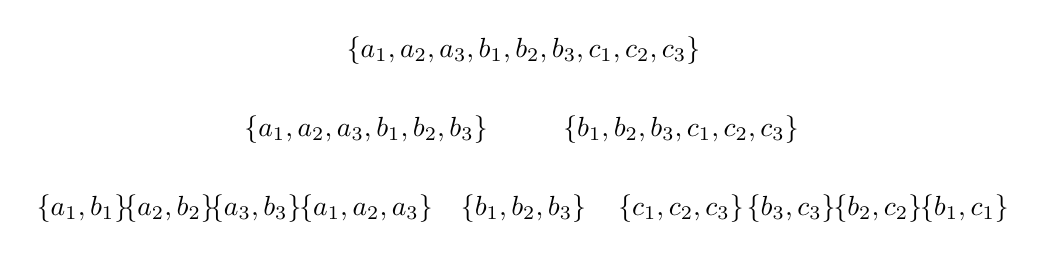
\begin{tikzpicture}
    \tikzstyle{v}=[draw, circle, minimum size=0.75cm]
    \tikzstyle{e}=[]

    \node (c0) at (0,0) {$\{a_1,a_2,a_3,b_1,b_2,b_3,c_1,c_2,c_3\}$};
    \node (c1a) at (-2,-1) {$\{a_1,a_2,a_3,b_1,b_2,b_3\}$};
    \node (c1b) at (2,-1) {$\{b_1,b_2,b_3,c_1,c_2,c_3\}$};
    \node (c2a) at (-2,-2) {$\{a_1,a_2,a_3\}$};
    \node (c2b) at (0,-2) {$\{b_1,b_2,b_3\}$};
    \node (c2c) at (2,-2) {$\{c_1,c_2,c_3\}$};
    \node (c2ab1) at (-5.6,-2) {$\{a_1,b_1\}$};
    \node (c2ab2) at (-4.5,-2) {$\{a_2,b_2\}$};
    \node (c2ab3) at (-3.4,-2) {$\{a_3,b_3\}$};
    \node (c2bc1) at (5.6,-2) {$\{b_1,c_1\}$};
    \node (c2bc2) at (4.5,-2) {$\{b_2,c_2\}$};
    \node (c2bc3) at (3.4,-2) {$\{b_3,c_3\}$};

    \tedge{c0}{c1a}{solid}{}{};
    \tedge{c0}{c1b}{solid}{}{};

    \tedge{c1a}{c2ab1}{solid}{}{};
    \tedge{c1a}{c2ab2}{solid}{}{};
    \tedge{c1a}{c2ab3}{solid}{}{};
    \tedge{c1a}{c2a}{solid}{}{};
    \tedge{c1a}{c2b}{solid}{}{};

    \tedge{c1b}{c2bc1}{solid}{}{};
    \tedge{c1b}{c2bc2}{solid}{}{};
    \tedge{c1b}{c2bc3}{solid}{}{};
    \tedge{c1b}{c2b}{solid}{}{};
    \tedge{c1b}{c2c}{solid}{}{};
\end{tikzpicture}

\caption{Two doublets ($C2\times C3$), $\{a_1,a_2,a_3,b_1,b_2,b_3\}$ and $\{b_1,b_2,b_3,c_1,c_2,c_3\}$, intersecting on the triangle $\{b_1,b_2,b_3\}$. Also showing the optimal DR-plan of the graph if we consider it to be a 2D graph; omits further decomposition of the three triangles into their edges and of edges into their individual nodes.}
\label{doublets}
\end{figure*}

\begin{example}
    In figure \ref{doublets}, the two well-constrained vertex-maximal proper subgraphs of the graph are the two doublets, shown in the second level of the DR-plan. These intersect on the well-constrained graph $\{b_1,b_2,b_3\}$. This will necessarily be a child $N=2$ levels below the parent of the two doublets, as explained in Theorem \ref{wc-t1}. Also shown is the decomposition of the individual doublets. These have five well-constrained vertex-maximal proper subgraphs, the two triangles and the three edges connecting them. As explained in Theorem \ref{uc-t1}, all of them must be included in the optimal DR-plan. Were any left out, the union of the children would not be the entire parent.
\end{example}



\begin{figure*}\centering
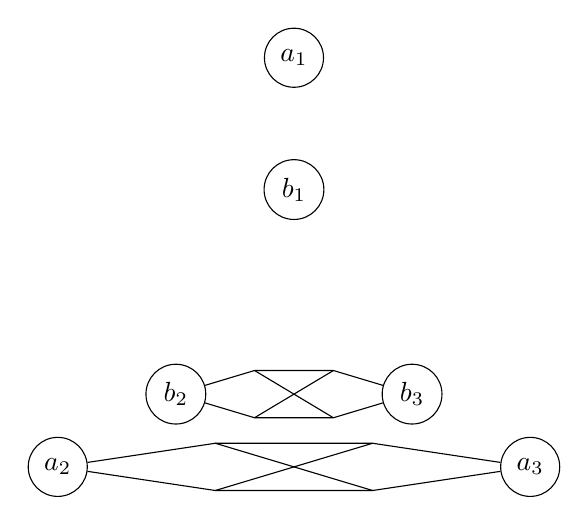
\begin{tikzpicture}[scale=3]
    \tikzstyle{v}=[draw, circle, minimum size=0.75cm]
    \tikzstyle{e}=[]

    \node[v] (v1) at (0,0.866) {$a_1$};
    \node[v] (v2) at (-1,-0.866) {$a_2$};
    \node[v] (v3) at (1,-0.866) {$a_3$};

    \node[v] (v4) at (0,0.433-.125) {$b_1$};
    \node[v] (v5) at (-0.5,-0.433-.125) {$b_2$};
    \node[v] (v6) at (0.5,-0.433-.125) {$b_3$};

    \tedge{v1}{v2}{solid}{}{};
    \tedge{v1}{v3}{solid}{}{};
    \tedge{v2}{v3}{solid}{}{};

    \tedge{v4}{v5}{solid}{}{};
    \tedge{v4}{v6}{solid}{}{};
    \tedge{v5}{v6}{solid}{}{};


    \tedge{v1}{v4}{solid}{}{};
    \tedge{v2}{v5}{solid}{}{};
    \tedge{v3}{v6}{solid}{}{};

    % sin(30deg) = 0.5
    % cos(30deg) = 0.866

    % o/i -> outside/inside triangle
    % b/l/r -> bottom/left/right edge of triangle

    \coordinate (ob0) at (-0.333,-0.866-0.1);
    \coordinate (ob1) at (0.333,-0.866-0.1);
    \coordinate (ob2) at (-0.333,-0.866+0.1);
    \coordinate (ob3) at (0.333,-0.866+0.1);
    \draw (v2) -- (ob0) -- (ob1) -- (v3);
    \draw (v2) -- (ob2) -- (ob3) -- (v3);
    \draw (ob0) -- (ob3);
    \draw (ob2) -- (ob1);

    \coordinate (ib0) at (-0.167,-0.433-.125-0.1);
    \coordinate (ib1) at (0.167,-0.433-.125-0.1);
    \coordinate (ib2) at (-0.167,-0.433-.125+0.1);
    \coordinate (ib3) at (0.167,-0.433-.125+0.1);
    \draw (v5) -- (ib0) -- (ib1) -- (v6);
    \draw (v5) -- (ib2) -- (ib3) -- (v6);
    \draw (ib0) -- (ib3);
    \draw (ib2) -- (ib1);



    % \draw[rotate around={60:(-1,-0.866)}] (v2) -- (-0.333,-0.766) -- (0.333,-0.766) -- (v1);
    % \draw (v2) -- (ob2) -- (ob3) -- (v1);
    % \draw (ob0) -- (ob3);
    % \draw (ob2) -- (ob1);
% \newcommand{\tedge}[5]{\draw[#3] (#1)-- node[e, #5] (e#4) {#4} (#2)}

    % \draw (-1,-0.866) -- (-0.333,-0.966);

\end{tikzpicture}

\caption{A doublet with each edge replaced by a $K3,3$. \todo{Drawing incomplete.}}
\label{c2c3ofk33s}
\end{figure*}

\begin{example}
    In figure \ref{c2c3ofk33s}... \todo{Is it worth working through this? The first example has trivial and non-trivial.}
\end{example}





\subsection{Extensions}
This framework immediately pushes through for body-pin systems via a simple reduction. If there are $N$ pins on a body, it can be represented as a 2-tree with $N$ vertices, each corresponding to a pin, making sure to select edge distances such that the distance between pins is preserved. E.g.\ a body with two pins is an edge, three pins is a triangle, etc. Any bodies that share a pin now intersect on their vertex that corresponds to that pin. Now we have a bar-joint representation of the body-pin system in 2D and all proofs follow.

With more effort, it can be shown that pinned line-incidence systems can also use this framework. This is done in section \ref{XXX}.



\subsection{Algorithm}
The algorithm to find the optimal DR-plan is a straightforward application of the theory. It begins by finding the well-constrained vertex-maximal proper subgraphs of the input well-constrained graph. If the intersection of any two of the subgraphs is well-constrained, then take those two to be children of the graph. Otherwise, all the subgraphs are the children. Apply recursively to the children. This naturally terminates when you reach trivial subgraphs.
